\chapter{Iteration 1: Design and Implementation}\label{ch:iter1}

\section{Iteration Objectives}
\begin{enumerate}
  \item \textbf{Architecture track:} design and implement a base architecture that keeps the map
        fast as images, models and layers grow, and prove it on the real AOI1 data.
  \item \textbf{Architecture track:} turn the prototype's ``upload and nothing happens'' into a real
        pipeline in which an uploaded image is analysed and published automatically.
  \item \textbf{Architecture track:} make models replaceable, so research results can be integrated
        without redesign.
  \item \textbf{Model track:} evaluate crop-type models under a fair spatial test, measure their cost,
        improve the best candidates, and compare with published work.
\end{enumerate}

\section{Selected Use Cases / Features}
\begin{table}[htbp]
\centering\small
\caption{Use cases and features selected for Iteration 1}
\label{tab:it1features}
\begin{tabularx}{\textwidth}{L{1.4cm} Y L{2.2cm}}
\toprule
\textbf{Use case} & \textbf{Feature} & \textbf{Track}\\
\midrule
UC-01, UC-02 & Tile-based Live Map with layer panel, legends, opacity, point inspection & Architecture\\
UC-03 & Crop filter, crop ranking and searchable field list & Architecture\\
UC-04 & Dashboard with pre-computed statistics and model accuracy & Architecture\\
UC-05, UC-06, UC-12 & Upload, background processing, live progress & Architecture\\
UC-07 & Re-analyse an existing image & Architecture\\
UC-08, UC-11 & Model catalogue and plug-in registry & Architecture\\
UC-09, UC-10 & Accounts and system status & Architecture\\
FR-MAP-02 & Crop-type model comparison, selection and error analysis & Model\\
\bottomrule
\end{tabularx}
\end{table}

\section{Design}
The architecture track implements the design of Chapter~5: Figure~\ref{fig:arch} (services),
Figure~\ref{fig:seq} (processing), Figure~\ref{fig:domain} and Table~\ref{tab:schema} (data). The
model track follows the experiment design in Figure~\ref{fig:experiment}: every experiment uses the
same inputs, split, classes and seed, and only the validation set decides.

\begin{figure}[htbp]
\centering
\begin{tikzpicture}[node distance=0.32cm, every node/.style={font=\scriptsize}]
\node[box, text width=2.05cm] (a) {\textbf{Inputs, labels}\\12 monthly S2 composites 2022; CDL 2022};
\node[box, text width=2.05cm, right=of a] (b) {\textbf{Spatial split}\\100$\times$100 px blocks 70/15/15, 3 px buffer};
\node[box, text width=2.05cm, right=of b] (c) {\textbf{Train}\\normalise on train; $\leq$30k px per class};
\node[box, text width=2.05cm, right=of c] (d) {\textbf{Validate}\\choose inputs, model, vote window};
\node[box, text width=2.05cm, right=of d] (e) {\textbf{Test, once}\\accuracy, macro-F1, per class, intervals};
\node[box, text width=2.05cm, right=of e] (f) {\textbf{Cost}\\CPU ms per 1000 px, size, RAM};
\draw[arr] (a)--(b); \draw[arr] (b)--(c); \draw[arr] (c)--(d); \draw[arr] (d)--(e); \draw[arr] (e)--(f);
\end{tikzpicture}
\caption{Crop-type experiment design}
\label{fig:experiment}
\end{figure}

\section{Implementation}
\textbf{Architecture track.} The platform was implemented as a new repository
(\code{geocrop-platform}) and runs as seven containers with Docker Compose: \code{web} (Nginx with
the built React app), \code{api} (FastAPI), \code{worker} (Celery), \code{tiles} (TiTiler),
\code{postgres} (PostGIS), \code{redis} and \code{minio}, plus a one-shot bucket initialiser.
Table~\ref{tab:loc} gives the size of each part. Data preparation scripts convert the AOI rasters to
COG, build the field-region PMTiles and load the AOI1 demonstration data.

\begin{table}[htbp]
\centering\small
\caption{Platform code by component (lines, including configuration and documentation)}
\label{tab:loc}
\begin{tabular}{L{4.0cm} L{6.6cm} r}
\toprule
\textbf{Component} & \textbf{Contents} & \textbf{Lines}\\
\midrule
\code{web/src} & React pages, map workspace, components, styles & 1,998\\
\code{backend/app} & API routes, models, services, workers, seed & 1,547\\
\code{backend/model_registry} & Contract, registry, graph, colour maps, models & 498\\
\code{ml} & Extended training scripts & 373\\
\code{docs} & Architecture, status, upgrade path, guides & 282\\
\code{tools} & COG conversion, boundaries, benchmark & 222\\
\code{tiles} & Tile service & 77\\
\code{infra} & Nginx and storage initialisation & 68\\
\bottomrule
\end{tabular}
\end{table}

\textbf{Model track.} Two notebooks implement the experiments: a benchmark notebook (runs 1 and 2,
model families, cost measurement, spatial bootstrap) and an accuracy-improvement notebook (run 3,
for AOI1 or AOI2). Inputs are 12 monthly Sentinel-2 composites of 2022 with 11 values per month
(B2, B3, B4, B5, B6, B7, B8, B8A, B11, B12 and NDVI) and the CDL 2022 rasters, all on the same 30~m
EPSG:5070 grid. AOI1 (eastern Washington, about 40$\times$37~km, 14 classes, 99,238 test pixels) is a
hard area with small fragmented fields, orchards and similar hay crops; AOI2 (north-eastern North
Dakota, about 38$\times$29~km, 9 classes, 144,922 test pixels) has large regular fields and two
dominant crops.

\section{Completed Features / Module}
\begin{table}[htbp]
\centering\small
\caption{Completed features at mid-term}
\label{tab:completed}
\begin{tabularx}{\textwidth}{L{3.8cm} Y L{1.4cm}}
\toprule
\textbf{Module} & \textbf{Completed} & \textbf{State}\\
\midrule
M1 Data preparation & COG conversion with validation; AOI1 Sentinel-2 composite and CDL as COG; monthly 2022 composites for AOI1 and AOI2 & Done\\
M2 Crop mapping & Platform: cropland and crop-type Random Forests trained and run on uploads. Research: 11 models compared; improved LightGBM pipeline selected & Done\\
M3 Field regions & 2,433 field regions (at least 25 pixels) as a 1.86~MB PMTiles layer and PostGIS rows & Interim\\
M4 Yield & Registered placeholder; NASS download script prepared & Planned\\
M5 Processing pipeline & Signed uploads, validation, reprojection, COG, background runs, progress, re-runs & Done\\
M6 Model registry & Contract, manifests, dependency graph, placeholders, NDVI template, add-a-model test & Done\\
M7 Catalogue and statistics & PostGIS schema with Alembic migration; zonal statistics; field search & Done\\
M8 Web GIS portal & Home, Live Map workspace, Dashboard, Analyze Imagery, Processing, Models, Status, accounts & Done\\
\bottomrule
\end{tabularx}
\end{table}

\section{Technical Implementation Details}
\begin{table}[htbp]
\centering\small
\caption{Important files, classes and functions}
\label{tab:files}
\begin{tabularx}{\textwidth}{L{5.3cm} Y}
\toprule
\textbf{File / element} & \textbf{Role}\\
\midrule
\code{model_registry/base.py}: \code{ModelTask}, \code{RunContext}, \code{RunResult}, \code{StubTask} & Contract every model implements; placeholders never fabricate data.\\
\code{model_registry/registry.py}: \code{Registry} & Scans folders for \code{manifest.yaml}, imports the entrypoint, isolates broken models.\\
\code{model_registry/graph.py}: \code{execution_order} & Topological order from required and produced layer kinds; readable errors for cycles and missing producers.\\
\code{builtin/cropland}, \code{builtin/croptype} & Windowed (512-pixel block) inference with saved models; crop type runs only on cropland pixels.\\
\code{app/workers/tasks.py}: \code{ingest_upload}, \code{run_pipeline} & Validate, reproject, convert, publish image; run models; publish layers and statistics; update job steps.\\
\code{app/services/layers.py}: \code{publish_raster_layer} & COG conversion, upload, footprint, layer row and zonal statistics in one step.\\
\code{app/services/rasters.py} & Footprint, point sampling, block-wise class statistics, reprojection to the model grid.\\
\code{app/services/vector_tiles.py} & Polygonise class rasters, simplify per zoom, encode MVT, write PMTiles.\\
\code{app/services/storage.py} & One storage interface for S3/MinIO and local disk; GDAL \code{/vsis3/} access.\\
\code{tiles/main.py} & Tile endpoint with server-side styles, crop filter, immutable caching.\\
\code{web/src/pages/LiveMap.tsx} & Map workspace; layers from the catalogue; filter, field search, inspection, tile traffic panel.\\
\code{docker-compose.yml}, \code{web/nginx.conf} & Services, health checks, tile cache, runtime DNS resolution.\\
\bottomrule
\end{tabularx}
\end{table}

Configuration is read from environment variables (\code{.env}); the database schema is created by an
Alembic migration that manages only GeoCrop's tables (the PostGIS image ships its own topology and
geocoder tables, which are excluded).

\section{Algorithms and Technical Decisions}
\subsection{Platform algorithms}
\begin{itemize}
  \item \textbf{COG conversion:} GDAL COG driver, 512-pixel blocks, DEFLATE, overviews with nearest
        neighbour for categorical rasters and average for imagery; validated by layout, tiling,
        overviews and CRS.
  \item \textbf{Tile rendering:} for tile $(z,x,y)$ the service reads the overlapping COG window at
        the matching overview, resamples (nearest for classes), maps class codes to the stored
        colours (optionally only selected classes) and encodes a PNG.
  \item \textbf{Windowed inference:} images are processed in 512$\times$512 windows; features follow
        the training composite (B2, B3, B4, B8, B11, B12, NDVI; NDVI computed when absent).
  \item \textbf{Dependency resolution:} depth-first topological sort over model manifests.
  \item \textbf{Zonal statistics:} block-wise class histograms; area = pixels $\times$ pixel area
        (900~m$^2$ = 0.09~ha at 30~m).
  \item \textbf{Field regions and PMTiles:} connected same-class regions of at least 25 pixels,
        simplified, encoded as MVT for zooms 8--14 (507 tiles) and packed into one PMTiles file.
\end{itemize}

\subsection{Crop-type evaluation protocol}\label{sec:protocol}
\begin{itemize}
  \item \textbf{Spatial block split:} whole 100$\times$100-pixel blocks go to training (70\%),
        validation (15\%) or test (15\%), with a 3-pixel buffer between them. A random pixel split
        leaks neighbours: on the same model it gave macro-F1 0.396 against 0.147 with blocks.
  \item Normalisation fitted on training pixels only; validation macro-F1 decides inputs, model and
        vote window; test results are computed once.
  \item Classes under 5,000 pixels are merged into ``Other (rare classes)''; up to 30,000 training
        pixels per class with balanced class weights; same split, classes and seed for every model.
  \item Cost is measured as CPU milliseconds per 1000 pixels, model size and RAM in a fresh
        single-thread process, as requested by the panel.
  \item Uncertainty: paired block bootstrap over the test blocks (4,000 resamples).
\end{itemize}

\subsection{Results: three runs on AOI1}
\begin{table}[htbp]
\centering\small
\caption{Progress over three runs on AOI1 (all test pixels)}
\label{tab:runs}
\begin{tabular}{c L{5.6cm} L{3.4cm} c c}
\toprule
\textbf{Run} & \textbf{Input} & \textbf{Model} & \textbf{Accuracy} & \textbf{Macro-F1}\\
\midrule
1 & One composite (single date) & Random Forest (3 seeds) & 0.267 & 0.191\\
2 & 12 monthly composites of 2022 & Random Forest (3 seeds) & 0.752 & 0.687\\
3 & + neighbourhood inputs + neighbour vote & Average of 3 models & 0.761 & 0.686\\
\bottomrule
\end{tabular}
\end{table}
Run 1 to 2 changed two things together: a time series instead of one date, and a satellite year that
matches the CDL year, so their separate effects are not known.

\begin{figure}[htbp]
\centering
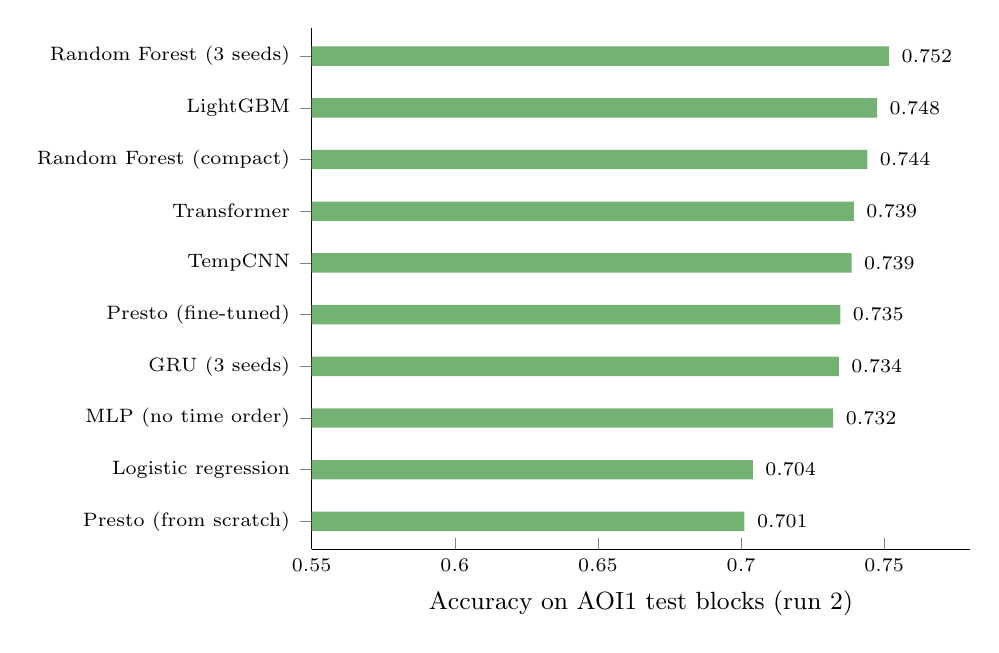
\begin{tikzpicture}
\begin{axis}[
  xbar, width=0.82\textwidth, height=8.2cm, xmin=0.55, xmax=0.78, bar width=7pt,
  ytick={0,...,9}, yticklabels={{Presto (from scratch)},{Logistic regression},{MLP (no time order)},{GRU (3 seeds)},{Presto (fine-tuned)},{TempCNN},{Transformer},{Random Forest (compact)},{LightGBM},{Random Forest (3 seeds)}},
  yticklabel style={font=\scriptsize}, xticklabel style={font=\scriptsize},
  xlabel={Accuracy on AOI1 test blocks (run 2)}, xlabel style={font=\small},
  nodes near coords, nodes near coords style={font=\scriptsize}, every node near coord/.append style={xshift=1pt},
  point meta=x, nodes near coords={\pgfmathprintnumber[fixed,precision=3]{\pgfplotspointmeta}},
  enlarge y limits=0.06, axis x line*=bottom, axis y line*=left]
\addplot[fill=green!45!black!55, draw=none] coordinates {
 (0.7012,0) (0.7041,1) (0.7322,2) (0.7342,3) (0.7347,4) (0.7386,5) (0.7394,6) (0.7441,7) (0.7475,8) (0.7517,9)};
\end{axis}
\end{tikzpicture}
\caption{Run 2: eleven models on the same AOI1 test blocks (axis starts at 0.55; majority class 0.199 not shown)}
\label{fig:models}
\end{figure}

Eight model families end within 2 points (73.2\% to 75.2\%); logistic regression is 4.8 points behind;
models that use time order (GRU, TempCNN~\cite{pelletier2019}, Transformer) do not clearly beat an MLP that ignores it.
Data and labels set the ceiling, not the algorithm, so the choice was made on cost
(Table~\ref{tab:cost}); LightGBM~\cite{ke2017} was proposed.

\begin{table}[htbp]
\centering\small
\caption{Accuracy against cost (run 2, AOI1; single-thread CPU)}
\label{tab:cost}
\begin{tabular}{L{4.2cm} r r r r}
\toprule
\textbf{Model} & \textbf{Accuracy} & \textbf{CPU ms / 1000 px} & \textbf{Size (MB)} & \textbf{RAM (MB)}\\
\midrule
Logistic regression & 0.704 & 0.016 & 1.2 & 321\\
MLP (no time order) & 0.732 & 3.8 & 0.29 & 550\\
Random Forest (compact) & 0.744 & 13.5 & 57.4 & 397\\
Random Forest (3 seeds) & 0.752 & 24.3 & 327.8 & 809\\
TempCNN & 0.739 & 31.9 & 0.6 & 570\\
\textbf{LightGBM (proposed)} & \textbf{0.748} & \textbf{35.8} & \textbf{1.98} & \textbf{549}\\
GRU (3 seeds) & 0.734 & 70.0 & 0.43 & 600\\
Transformer & 0.739 & 79.9 & 0.29 & 588\\
Presto (fine-tuned) & 0.735 & 2551 & 1.65 & 1200\\
\bottomrule
\end{tabular}
\end{table}

\subsection{Run 3: improvement ladder}
An improvement was kept only if validation macro-F1 rose by at least 0.002.
\begin{table}[htbp]
\centering\small
\caption{Improvement ladder (inputs per month; AOI1 validation change; AOI2 scores)}
\label{tab:ladder}
\begin{tabular}{L{4.1cm} c L{2.0cm} c c c}
\toprule
\textbf{Step} & \textbf{Inputs} & \textbf{AOI1 val.} & \textbf{AOI2 val.} & \textbf{AOI2 test} & \textbf{Decision}\\
 & \textbf{/ month} & \textbf{change} & \textbf{macro-F1} & \textbf{accuracy} & \\
\midrule
0 Benchmark (raw inputs) & 11 & start & 0.731 & 0.903 & start\\
1 + 4 indices, month flag & 16 & +0.0017 & 0.695 & 0.889 & dropped\\
2 + cleaned training labels & 11 & $-$0.030 & 0.681 & 0.909 & dropped\\
3 + neighbourhood inputs & 19 & +0.0024 & 0.742 & 0.912 & kept\\
\bottomrule
\end{tabular}
\end{table}
Neighbourhood inputs are the mean of NDVI, B8 and B11 over 3$\times$3 and 7$\times$7 windows and the spread
of NDVI; the 7$\times$7 window reaches 3 pixels, equal to the buffer, so no training pixel overlaps a
test block. Cleaning labels (removing edge pixels from training) hurt, because 29--47\% of test pixels
are edge pixels. The 3$\times$3 neighbour vote averages predicted probabilities of nearby test pixels;
window 3 was best on validation in both areas.

\subsection{Run 3 results in both areas}
\begin{table}[htbp]
\centering\small
\caption{Final results on both areas (all test pixels)}
\label{tab:both}
\begin{tabular}{L{6.2cm} c c}
\toprule
 & \textbf{AOI1 (E. Washington)} & \textbf{AOI2 (NE North Dakota)}\\
\midrule
Classes / test pixels & 14 / 99,238 & 9 / 144,922\\
Benchmark: accuracy / macro-F1 & 0.741 / 0.661 & 0.903 / 0.759\\
Improved inputs & 0.756 / 0.685 & 0.912 / 0.780\\
Improved + neighbour vote & \textbf{0.761 / 0.686} & \textbf{0.922 / 0.803}\\
Gain over benchmark (points) & +2.0 / +2.5 & +1.8 / +4.4\\
Test pixels on field edges & 47.0\% & 29.4\%\\
Accuracy on interior / edge pixels & 0.952 / 0.546 & 0.988 / 0.762\\
Share of errors on edge pixels & 89\% & 89\%\\
Final model (chosen on validation) & Average of 3 models & LightGBM\\
\bottomrule
\end{tabular}
\end{table}

\begin{figure}[htbp]
\centering
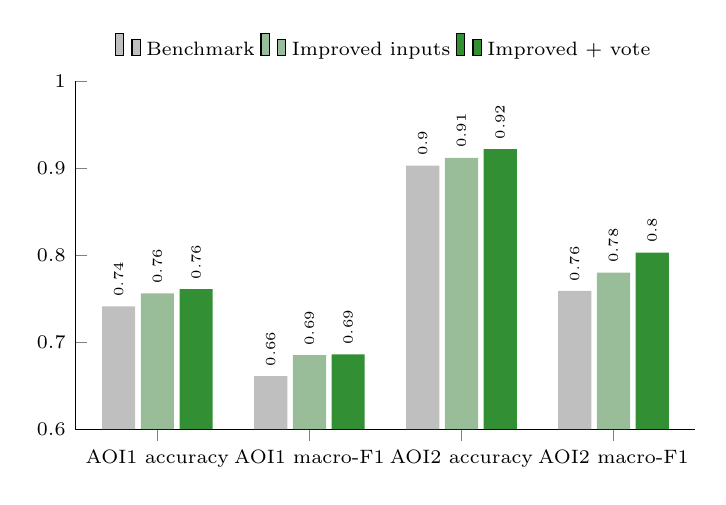
\begin{tikzpicture}
\begin{axis}[
  ybar, width=0.78\textwidth, height=6.0cm, ymin=0.6, ymax=1.0, bar width=12pt,
  symbolic x coords={AOI1 accuracy,AOI1 macro-F1,AOI2 accuracy,AOI2 macro-F1}, xtick=data,
  xticklabel style={font=\scriptsize}, yticklabel style={font=\scriptsize},
  legend style={font=\scriptsize, at={(0.5,1.03)}, anchor=south, legend columns=3, draw=none},
  nodes near coords, nodes near coords style={font=\tiny, rotate=90, anchor=west},
  enlarge x limits=0.18, axis x line*=bottom, axis y line*=left]
\addplot[fill=black!25, draw=none] coordinates {(AOI1 accuracy,0.741) (AOI1 macro-F1,0.661) (AOI2 accuracy,0.903) (AOI2 macro-F1,0.759)};
\addplot[fill=green!35!black!40, draw=none] coordinates {(AOI1 accuracy,0.756) (AOI1 macro-F1,0.685) (AOI2 accuracy,0.912) (AOI2 macro-F1,0.780)};
\addplot[fill=green!45!black!80, draw=none] coordinates {(AOI1 accuracy,0.761) (AOI1 macro-F1,0.686) (AOI2 accuracy,0.922) (AOI2 macro-F1,0.803)};
\legend{Benchmark, Improved inputs, Improved + vote}
\end{axis}
\end{tikzpicture}
\caption{Benchmark, improved inputs and neighbour vote in both areas (axis starts at 0.6)}
\label{fig:both}
\end{figure}

\textbf{How to quote the result.} AOI1: 76.1\% on all test pixels (95\% interval 72.1\% to 79.6\% over
test blocks), macro-F1 0.686; on field interiors 95.2\%. The improved pipeline is +2.0 points over the
benchmark (interval +1.0 to +3.0). Run-to-run noise is about 0.7 points, so differences under about
1 point are not reliable.

\textbf{Error analysis.} About 89\% of errors in both areas sit on pixels that touch another label;
67\% of AOI1 edge errors predict the neighbouring class (boundary bleed). Confusions are between
agronomically close classes: Alfalfa and Other Hay, Corn and Sweet Corn (AOI1); Spring Wheat and
Barley, Spring Wheat and Fallow/Idle (AOI2). Weakest AOI1 classes by F1 are Fallow/Idle (0.29) and
Other (0.29); strongest are Onions (0.91), Potatoes (0.86) and Alfalfa (0.85)
(Appendix~\ref{app:tests}, Table~\ref{tab:perclass}).

\subsection{Comparison with published work}\label{sec:papers}
\begin{table}[htbp]
\centering\small
\caption{GeoCrop crop-type results next to published studies (context, not a ranking)}
\label{tab:papers}
\begin{tabularx}{\textwidth}{L{2.8cm} L{1.6cm} L{3.3cm} Y L{1.9cm}}
\toprule
\textbf{Study} & \textbf{Unit} & \textbf{Labels / split} & \textbf{Result} & \textbf{Classes}\\
\midrule
GeoCrop (ours) & Pixel, 30~m & CDL 2022, all pixels; spatial blocks & AOI2 92.2\%; AOI1 76.1\% (interior 95.2\%) & 9 and 14\\
Tran et al.\ 2022~\cite{tran2022} & Pixel, 10~m & Good-quality CDL; 80/20 samples & 94\% South Dakota; 83\% California & 10 and 20\\
Li et al.\ 2024~\cite{li2024} & Pixel & Trusted CDL pixels & Corn/soybean F1 0.85--0.97 & --\\
PSE-TAE 2020~\cite{garnot2020} & Parcel & Parcel declarations & OA 94.2\%; RF 91.6\% & 20\\
BreizhCrops 2020~\cite{russwurm2020} & Parcel & Held-out region & Transformer 0.81, TempCNN 0.80, RF 0.78 & 9\\
Presto 2023~\cite{tseng2023} & Pixel series & Pre-trained & S2-Agri100 OA 68.9\% & --\\
Prithvi-EO-2.0 2024~\cite{szwarcman2024} & Chip & CDL, 3 dates & mIoU 48.6--50.7 & 13\\
\bottomrule
\end{tabularx}
\end{table}
AOI2 (92.2\%) is close to the 94\% reported for South Dakota, a similar northern-plains crop mix,
while using a stricter spatial split and no label-quality filter. AOI1 (76.1\%) is below the 83\% for
California but is a harder area with 47\% edge pixels. Parcel-level studies classify whole fields,
which removes the edge problem, so their numbers are not directly comparable. As in the papers, the
algorithm moves results by a few points, while labels and the evaluation unit move them by tens of
points. A like-for-like comparison needs the CDL confidence filter and matching class sets
(Iteration~2).

\textbf{Baseline model in the platform.} The platform currently runs the proposal-stage two-stage
Random Forest (single composite, seven features), retrained and saved for live inference. Its
held-out scores of 93\% (cropland) and 56\% (crop type) come from a random pixel split and are shown
in the portal with that caveat; under the spatial protocol a single-date input reaches only 26.7\%.
Replacing it with the selected pipeline is the first task of Iteration~2.

\section{Tools, Frameworks and Technologies}
\begin{table}[htbp]
\centering\small
\caption{Tools, frameworks and technologies}
\label{tab:tools}
\begin{tabularx}{\textwidth}{L{3.2cm} Y}
\toprule
\textbf{Area} & \textbf{Tools}\\
\midrule
Frontend & React 19, Vite, TypeScript, MapLibre GL JS, react-map-gl, pmtiles, TanStack Query, Zustand, React Router\\
Backend & Python 3.12, FastAPI, Pydantic, SQLAlchemy 2, GeoAlchemy2, Alembic, PyJWT, bcrypt, boto3\\
Geospatial & GDAL/rasterio, rio-tiler, TiTiler, shapely, pyproj, mercantile, mapbox-vector-tile, PostGIS 3.4\\
Processing & Celery, Redis 7\\
Storage & MinIO (S3 API), PostgreSQL 16\\
Machine learning & scikit-learn, LightGBM, PyTorch (deep models in the comparison), Presto, joblib, NumPy\\
Data & Google Earth Engine (Sentinel-2 export), USDA CDL, USDA NASS QuickStats\\
DevOps & Docker, Docker Compose, Nginx, Git\\
Testing & pytest, curl-based API checks, headless browser checks, custom tile benchmark\\
\bottomrule
\end{tabularx}
\end{table}

\section{Demonstration Evidence}\label{sec:demo}
\textbf{Rendering benchmark.} Table~\ref{tab:benchmark} compares the prototype's approach with the new
tile path on the same AOI1 crop-type result, measured through Nginx on a laptop.

\begin{table}[htbp]
\centering\small
\caption{Rendering benchmark on AOI1 (crop-type layer, zoom 12)}
\label{tab:benchmark}
\begin{tabularx}{\textwidth}{L{4.6cm} Y Y}
\toprule
\textbf{Measure} & \textbf{Prototype (GeoJSON)} & \textbf{GeoCrop (COG tiles)}\\
\midrule
Data for one screen of AOI1 & 43.3~MB (whole file) & 337~KB (24 tiles)\\
Objects the browser draws & 101,435 polygons ($\approx$750k vertices) & 24 PNG images\\
Server / parse time & 1,021~ms to parse the JSON only & cold tile median 47~ms, p95 54~ms\\
Cached tile latency & no caching & median 1~ms (Nginx hit)\\
Typical tile size & n/a & median 2.9~KB, max 44~KB\\
Storage of the same result & 43.3~MB GeoJSON & 222~KB compressed GeoTIFF\\
\bottomrule
\end{tabularx}
\end{table}

\begin{figure}[htbp]
\centering
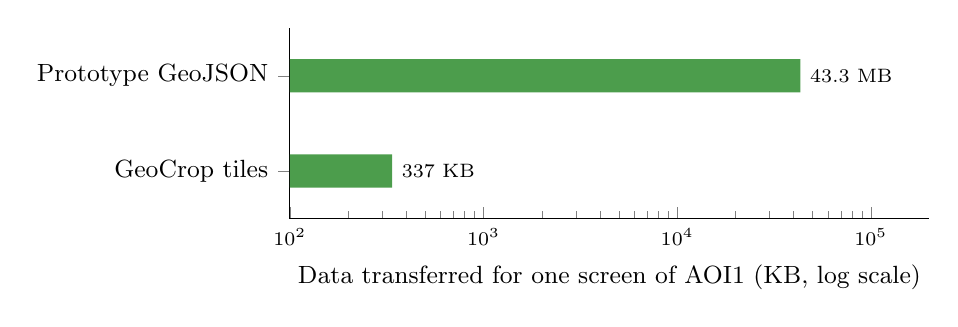
\begin{tikzpicture}
\begin{axis}[xbar, xmode=log, width=0.8\textwidth, height=4.0cm, bar width=12pt,
  symbolic y coords={GeoCrop tiles,Prototype GeoJSON}, ytick=data,
  xlabel={Data transferred for one screen of AOI1 (KB, log scale)}, xlabel style={font=\small},
  yticklabel style={font=\small}, xticklabel style={font=\scriptsize}, xmin=100, xmax=200000,
  enlarge y limits=0.5, axis x line*=bottom, axis y line*=left]
\addplot[fill=green!45!black!70, draw=none] coordinates {(337,GeoCrop tiles) (43300,Prototype GeoJSON)};
\node[anchor=west, font=\scriptsize] at (axis cs:337,GeoCrop tiles) {337 KB};
\node[anchor=west, font=\scriptsize] at (axis cs:43300,Prototype GeoJSON) {43.3 MB};
\end{axis}
\end{tikzpicture}
\caption{Data per screen: prototype against tile-based delivery (about 130 times less)}
\label{fig:benchmark}
\end{figure}

\textbf{Pipeline run.} Uploading the AOI1 Sentinel-2 GeoTIFF through a signed URL, ingesting it,
running the cropland and crop-type models block by block and publishing both layers took 57~s,
with each step visible on the Processing page. Loading the AOI1 demonstration data took about 5~s.

\textbf{Screenshots.} Figures~\ref{fig:shot-home}--\ref{fig:shot-status} show the running portal.

\begin{figure}[htbp]
\centering
\fbox{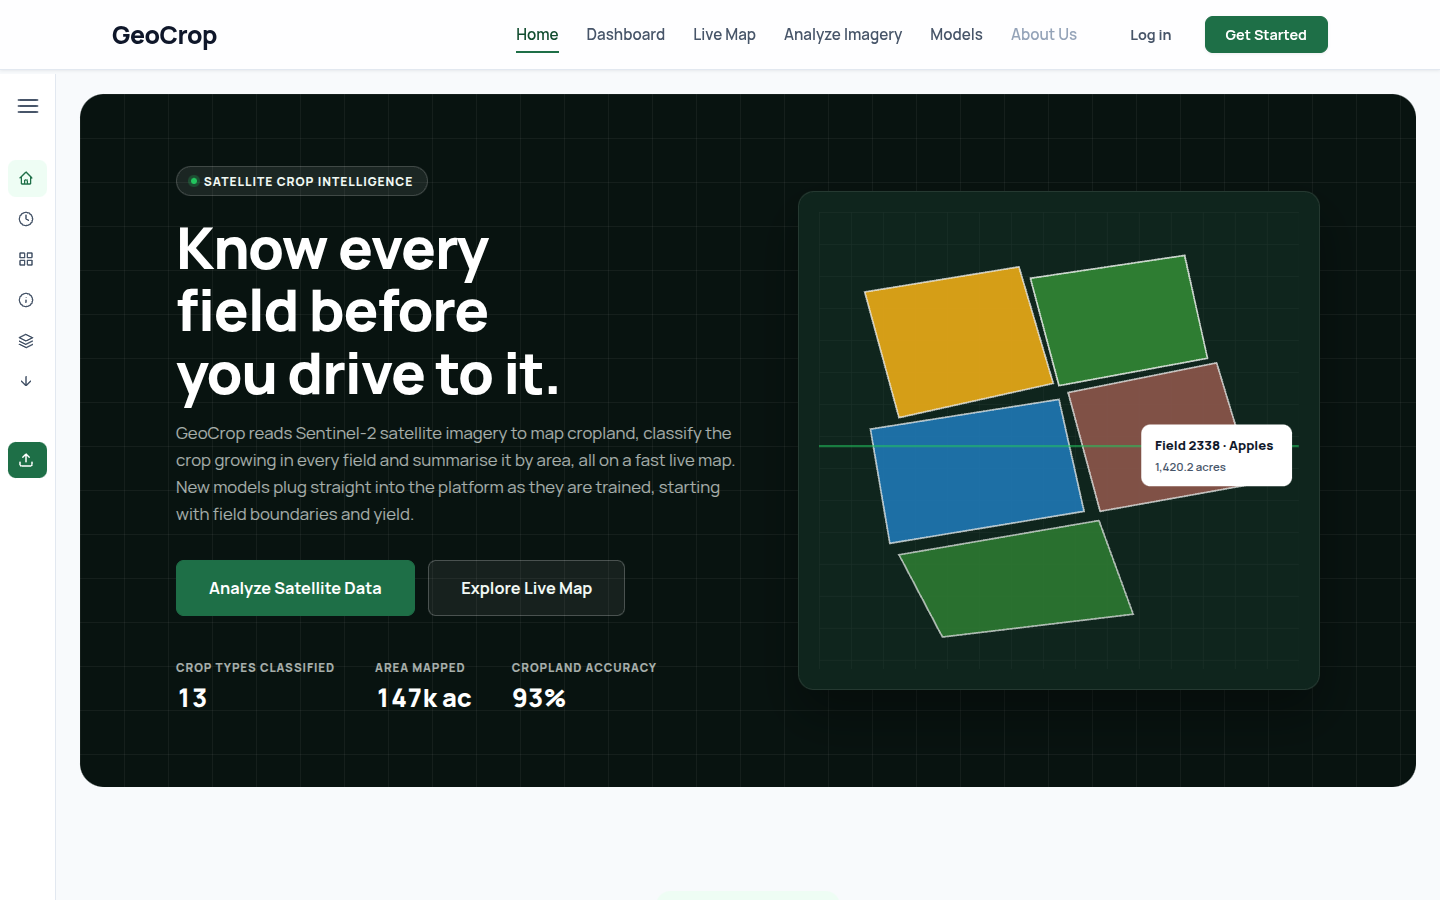
\includegraphics[width=0.92\textwidth]{figures/shot_home.png}}
\caption{Home page with live figures from the AOI1 results}
\label{fig:shot-home}
\end{figure}

\begin{figure}[htbp]
\centering
\fbox{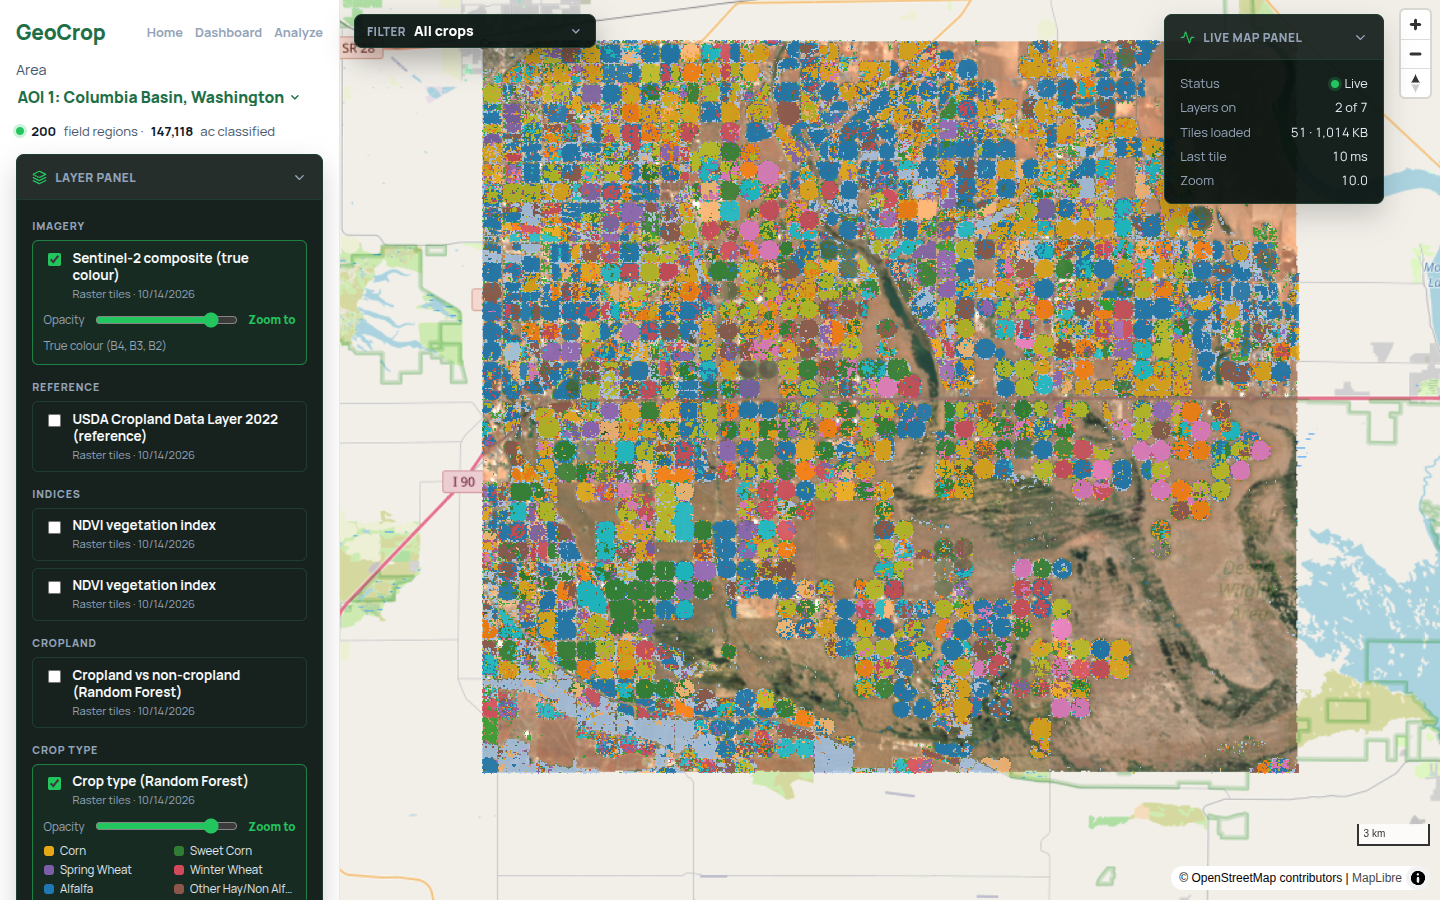
\includegraphics[width=0.92\textwidth]{figures/shot_map.png}}
\caption{Live Map workspace: layer panel, crop-type layer over Sentinel-2 imagery, crop filter and Live map panel (tiles loaded and latency)}
\label{fig:shot-map}
\end{figure}

\begin{figure}[htbp]
\centering
\fbox{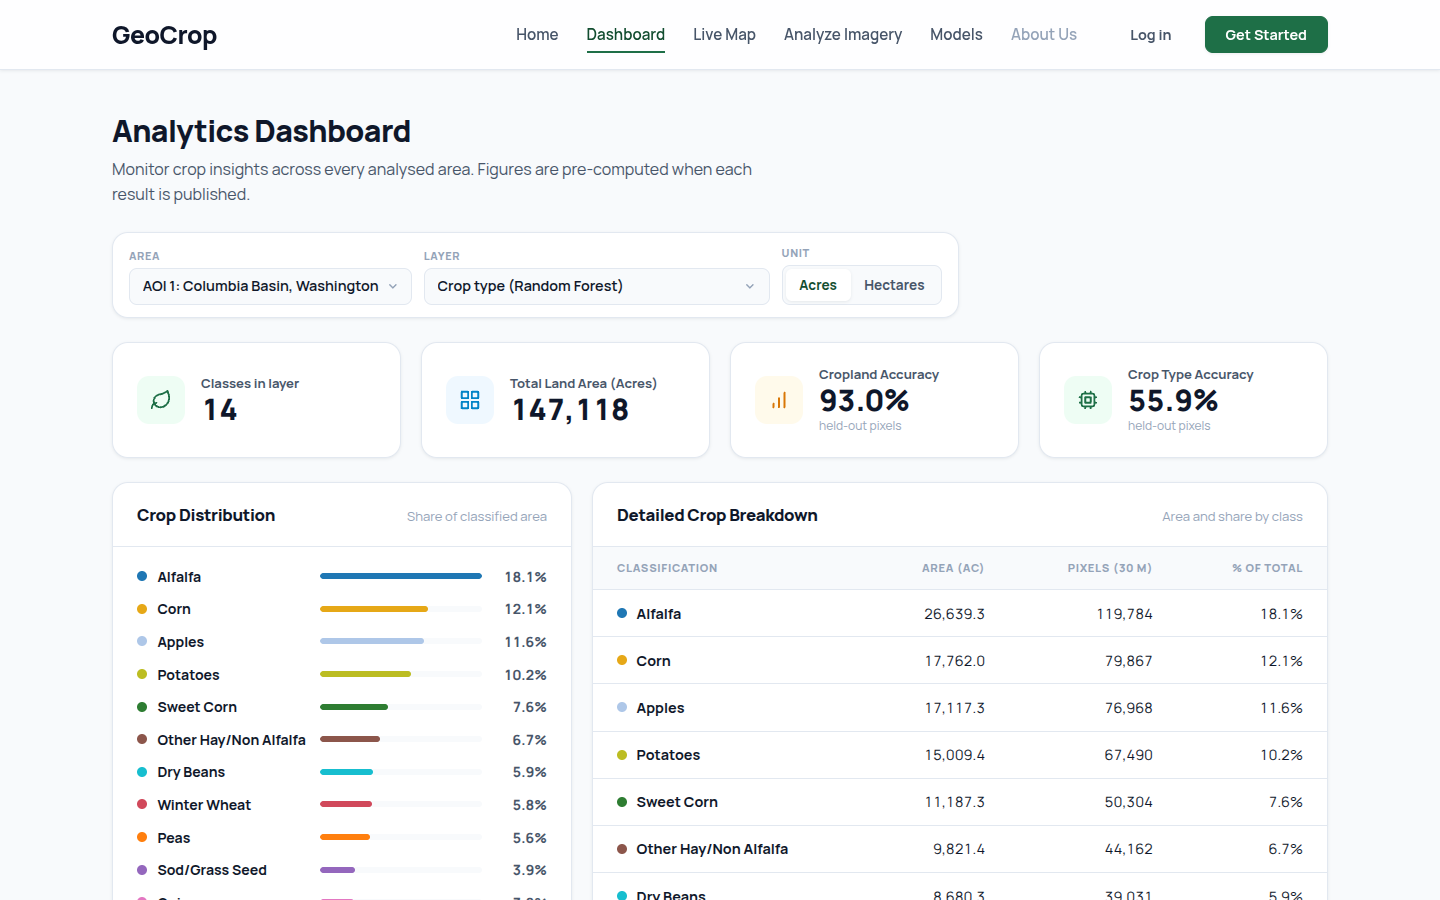
\includegraphics[width=0.92\textwidth]{figures/shot_dashboard.png}}
\caption{Analytics Dashboard: statistics from PostGIS and measured model accuracy}
\label{fig:shot-dashboard}
\end{figure}

\begin{figure}[htbp]
\centering
\fbox{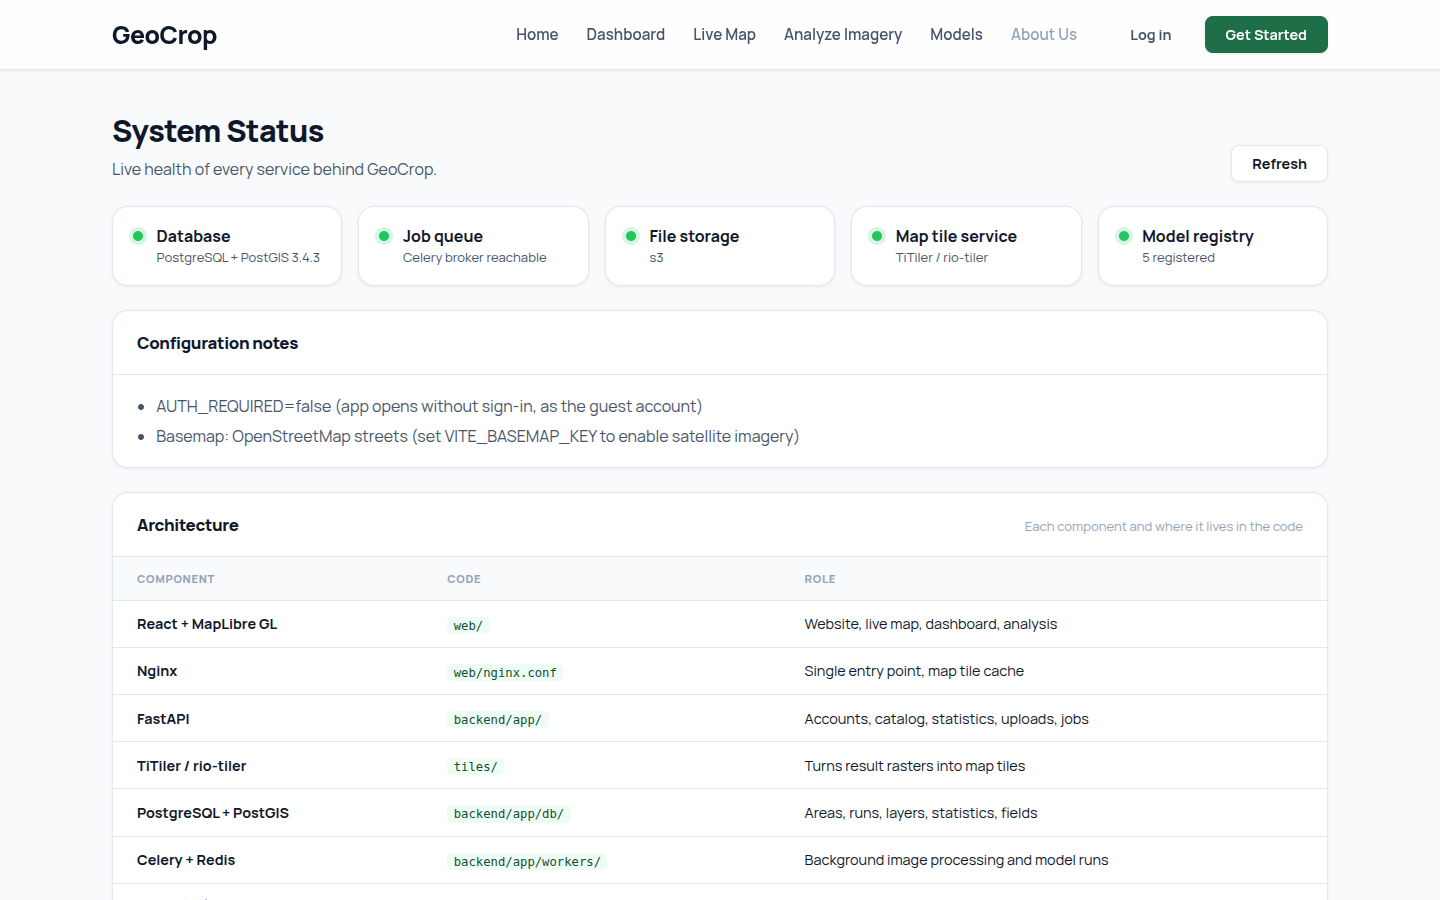
\includegraphics[width=0.92\textwidth]{figures/shot_status.png}}
\caption{System Status: health of every service and the architecture map}
\label{fig:shot-status}
\end{figure}

\subsection{Workflow feasibility and resource requirements}\label{sec:feasibility}
The panel found that the complexity and resource requirements of the complete workflow had not been
analysed, and that running it as one single flow may not be practical (P4, P5). Each stage was
therefore measured on its own on the AOI1 image (1,332$\times$1,239 pixels at 30~m, about
148,500~ha, 7 inputs per pixel). Every stage ran in a fresh process in the worker container, on an
8-core laptop CPU with 15~GB RAM, reading the image in 512$\times$512 blocks
(Table~\ref{tab:resources}).

\begin{table}[htbp]
\centering\small
\caption{Measured resource requirements of the complete workflow (AOI1, one fresh process per stage)}
\label{tab:resources}
\begin{tabularx}{\textwidth}{L{3.6cm} r r Y}
\toprule
\textbf{Stage} & \textbf{Time} & \textbf{Peak RAM} & \textbf{Storage / notes}\\
\midrule
Upload and validation & -- & -- & Input GeoTIFF 24.8~MB, sent directly to object storage\\
Cloud-optimised GeoTIFF & 0.7~s & 357~MB & 29.5~MB COG with overviews\\
Cropland model (RF) & 1.1~s load + 2.7~s & 395~MB & Model 71.6~MB; 1.11~M pixels classified\\
Crop-type model (baseline RF) & 2.5~s load + 7.5~s & \textbf{3,145~MB} & Model \textbf{1.57~GB}; 0.69~M cropland pixels\\
Crop-type model (LightGBM, proposed) & 35.8~ms / 1000~px & 549~MB & Model 1.98~MB (Table~\ref{tab:cost})\\
Publish results & -- & -- & Crop type 222~KB, cropland 63~KB compressed rasters; statistics in PostGIS\\
Full upload-to-map run & 57~s & -- & Includes transfer, queueing, storage writes and publishing\\
Idle platform (7 services) & -- & about 1.0~GB & Database 23~MB with AOI1 loaded\\
\bottomrule
\end{tabularx}
\end{table}

Three findings follow. First, the compute itself is small: all model and conversion stages together
take about 15~s; the rest of the 57~s run is transfer, queueing and publishing. Second, memory, not
time, is the real limit. The baseline Random Forest crop-type model needs 1.57~GB on disk and about
3.1~GB of RAM, so two parallel runs would already need more than 6~GB. The proposed LightGBM model
needs 549~MB (measured by the model track, Table~\ref{tab:cost}) at about the same accuracy, which makes the full workflow fit on a normal laptop.
Third, results are small once stored as compressed rasters (285~KB for both layers against 43.3~MB
of GeoJSON), so storage grows slowly as AOIs and models are added.

The design therefore avoids a single flow. Ingest, each model and publishing are separate queued
steps that run in background workers, one model at a time in dependency order, with progress and
errors recorded per step. A failed or heavy step does not block the map, the API or other jobs, and
workers can be added on another machine without changing the code. Users never load the whole
dataset: the map requests only the tiles in view.

\section{Iteration Outcome}
Iteration 1 met its objectives. The architecture track delivered a working platform that reduces the
data for one screen from 43.3~MB to 337~KB, serves cold tiles in 47~ms and cached tiles in 1~ms,
analyses uploaded imagery end to end in under a minute, and accepts new models by folder and
manifest. The model track established a fair evaluation protocol, showed that a time series is the
key input and that model family matters little, selected a small CPU-only LightGBM pipeline
(76.1\% AOI1, 92.2\% AOI2) and located the remaining errors on field edges. Measuring every workflow stage answered the panel's feasibility question: compute is small,
memory is the limit, and the selected LightGBM model removes the 3.1~GB bottleneck of the baseline.
The main open items are
integrating the selected pipeline into the platform, the CDL confidence rule, the cross-area test,
and the boundary and yield models.
